\section{What is Sound?}

\frame{\tableofcontents[currentsection]}

\begin{frame}
  \frametitle{Sound}
  \begin{itemize}
    \item Sound is a vibration
    \item Goes up and down in time
    \item Can be represented mathematically by a function $\mathbb{R} \rightarrow \mathbb{R}$
    \item In code: \texttt{double sound(double t)}
          \begin{itemize}
            \item Parameter \texttt{t}: time
            \item Return value: amplitude at time \texttt{t}
          \end{itemize}
  \end{itemize}
  \begin{center}
    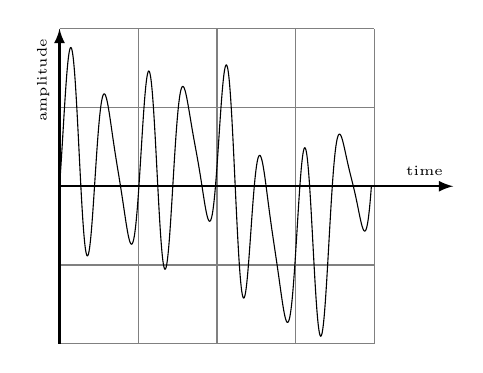
\begin{tikzpicture}[label/.style={font=\tiny}]
      \draw[thin,gray] (0,-2) grid (4,2);
      \draw[thin] plot[domain=0:360,x=0.011cm,y=1cm,samples=1000,smooth] (\x,{sin(8*\x)+0.75 * sin(7*\x)*sin(5*\x)+0.5*sin(\x)});
      \draw[-latex,thick] (0,0) -- ++(5,0) node[anchor=south east,label] {time};
      \draw[-latex,thick] (0,-2) -- (0,2) node[anchor=south east,label,rotate=90] {amplitude};
    \end{tikzpicture}
  \end{center}
\end{frame}

\subsection{Pitch}

\frame{\tableofcontents[currentsubsection]}

\begin{frame}
  \frametitle{Frequency - Pitch}
  \begin{itemize}
    \item Sound is characterised by its frequency
    \item Frequency = how many vibrations per second
    \item Low frequency = low pitch
    \item High frequency = high pitch
  \end{itemize}
  \begin{center}
    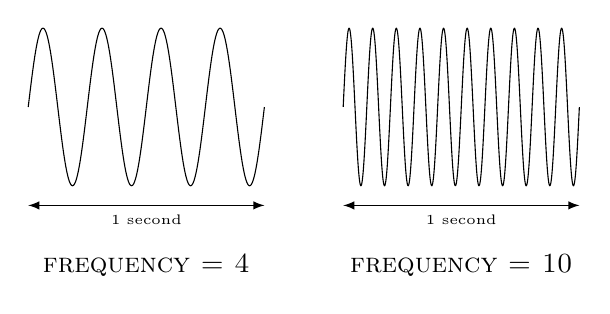
\begin{tikzpicture}
      \begin{scope}
        \draw[thin] plot[domain=0:360,x=0.00833cm,y=1cm,samples=1000,smooth] (\x,{sin(4*\x)});
        \node[anchor=north,font=\scshape] at (1.5,-1.75) {frequency = 4};
        \draw[latex-latex] (0,-1.25) -- ++(3,0) node[below,font=\tiny,midway] {1 second};
      \end{scope}

      \begin{scope}[xshift=4cm]
        \draw[thin] plot[domain=0:360,x=0.00833cm,y=1cm,samples=1000,smooth] (\x,{sin(10*\x)});
        \node[anchor=north,font=\scshape] at (1.5,-1.75) {frequency = 10};
        \draw[latex-latex] (0,-1.25) -- ++(3,0) node[below,font=\tiny,midway] {1 second};
      \end{scope}
    \end{tikzpicture}
  \end{center}
\end{frame}

\begin{frame}
  \frametitle{Notes}
  \begin{center}
    \begin{tabular}{ccc}
      \textbf{Letter} & \textbf{Note} & \textbf{Frequency} \\
      \toprule
      C & do & 261.63 \\
      D & re & 293.66 \\
      E & mi & 329.63 \\
      F & fa & 349.23 \\
      G & sol & 392.00 \\
      A & la & 440.00 \\
      B & si & 493.88 \\
      \bottomrule
    \end{tabular}
  \end{center}
\end{frame}

\subsection{Loudness}

\frame{\tableofcontents[currentsubsection]}

\begin{frame}
  \frametitle{Amplitude - Loudness}
  \begin{itemize}
    \item Sound is also characterised by its amplitude
    \item Amplitude = how far up and down the wave goes
    \item Small amplitude = soft
    \item Large amplitude = loud
  \end{itemize}
  \begin{center}
    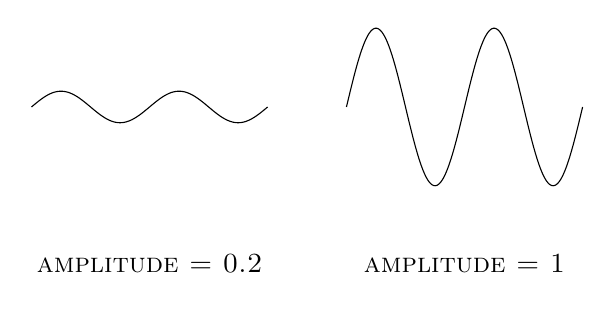
\begin{tikzpicture}
      \begin{scope}
        \draw[thin] plot[domain=0:360,x=0.00833cm,y=1cm,samples=1000,smooth] (\x,{0.2*sin(2*\x)});
        \node[anchor=north,font=\scshape] at (1.5,-1.75) {amplitude = 0.2};
      \end{scope}

      \begin{scope}[xshift=4cm]
        \draw[thin] plot[domain=0:360,x=0.00833cm,y=1cm,samples=1000,smooth] (\x,{sin(2*\x)});
        \node[anchor=north,font=\scshape] at (1.5,-1.75) {amplitude = 1};
      \end{scope}
    \end{tikzpicture}
  \end{center}
\end{frame}

\subsection{Timbre}

\frame{\tableofcontents[currentsubsection]}

\begin{frame}
  \frametitle{Waveform - Timbre}  
  \begin{center}
    \begin{tabular}{cccc}
      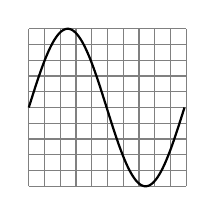
\begin{tikzpicture}
        \draw[thin,gray] (0,-1) grid[xstep=2mm,ystep=2mm] (2,1);
        \draw[thick] plot[domain=0:360,x=0.0055cm,y=1cm,samples=1000,smooth] (\x,{sin(\x)});
      \end{tikzpicture}
      &
      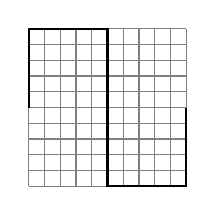
\begin{tikzpicture}
        \draw[thin,gray] (0,-1) grid[xstep=2mm,ystep=2mm] (2,1);
        \draw[thick] (0,0) -- ++(0,1) -- ++(1,0) -- ++(0,-2) -- ++(1,0) -- ++(0,1);
      \end{tikzpicture}
      &
      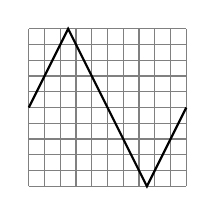
\begin{tikzpicture}
        \draw[thin,gray] (0,-1) grid[xstep=2mm,ystep=2mm] (2,1);
        \draw[thick] (0,0) -- (0.5,1) -- (1.5,-1) -- (2,0);
      \end{tikzpicture}
      &
      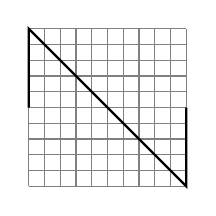
\begin{tikzpicture}
        \draw[thin,gray] (0,-1) grid[xstep=2mm,ystep=2mm] (2,1);
        \draw[thick] (0,0) -- (0,1) -- (2,-1) -- (2,0);
      \end{tikzpicture}
      \\
      \textbf{Sine} & \textbf{Square} & \textbf{Triangle} & \textbf{Sawtooth}
    \end{tabular}
  \end{center}
  \begin{itemize}
    \item Any shape can be used to produce sound
    \item Each shape has its own sound
    \item Simple shapes are reminiscent of old games
    \item Musical instruments correspond to different shapes
    \item \link{http://meettechniek.info/additional/additive-synthesis.html}{Experiment online}
  \end{itemize}
\end{frame}

\subsection{Composing Music}

\frame{\tableofcontents[currentsubsection]}

\begin{frame}
  \frametitle{How to Compose Music}
  \begin{itemize}
    \item Choose an ``instrument''
          \begin{itemize}
            \item I.e.~choose a waveform
            \item Sine is both pleasant and simple
          \end{itemize}
    \item Choose which notes to play
          \begin{itemize}
            \item E.g.~do re miiii
          \end{itemize}
    \item Put the corresponding waves in the right order
  \end{itemize}
  \begin{center}
    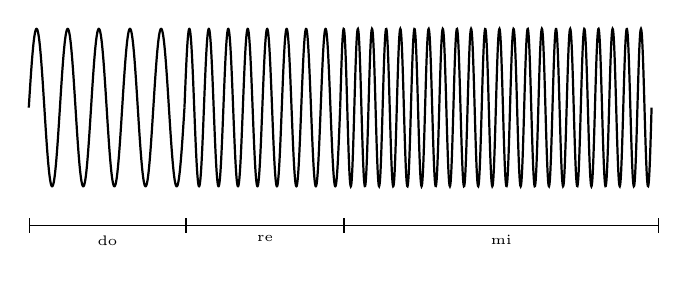
\begin{tikzpicture}
      \draw[thick] plot[domain=0:360,x=0.0055cm,y=1cm,samples=1000,smooth] (\x,{sin(5*\x)});
      \draw[thick] plot[domain=360:720,x=0.0055cm,y=1cm,samples=1000,smooth] (\x,{sin(8*\x)});
      \draw[thick] plot[domain=720:1440,x=0.0055cm,y=1cm,samples=1000,smooth] (\x,{sin(11*\x)});
      \draw[|-|] (0,-1.5) -- ++(2,0) node[below,midway,font=\tiny] {do};
      \draw[|-|] (2,-1.5) -- ++(2,0) node[below,midway,font=\tiny] {re};
      \draw[|-|] (4,-1.5) -- ++(4,0) node[below,midway,font=\tiny] {mi};
    \end{tikzpicture}
  \end{center}
\end{frame}



%%% Local Variables:
%%% mode: latex
%%% TeX-master: "sound"
%%% End:
